\section*{Pregunta 6}
\noindent Let $P$ be a set of $n$ points in the plane. The staircase of $P$ is the set of all points in the plane that have at least one point in $P$ both above and to the right.
\begin{center}
    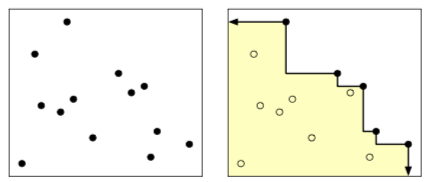
\includegraphics[scale=0.5]{escalera1}
\end{center}

\begin{enumerate}
    \item Describe an algorithm to compute the staircase of a set of $n$ points in $O(n \log n)$ time.
    
    \item Describe and analyze a data structure that stores the staircase of a set of points, and an algorithm ABOVE? $(x, y)$ that returns \textsc{true} if the point $(x, y)$ is above the staircase, or \textsc{fals} otherwise. Your data structure should use $O(n)$ space, and your ABOVE? algorithm should run in $O(log n)$ time.
\end{enumerate}

\begin{center}
    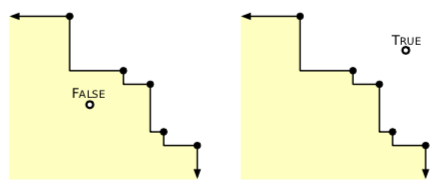
\includegraphics[scale=0.5]{escalera2}
\end{center}

\subsection*{Respuesta}
\begin{enumerate}
    \item Describe an algorithm to compute the staircase of a set of $n$ points in $O(n \log n)$ time.
    \begin{algorithmic}[1]
        \State escalera=$\{\}$
        \State Ordenar los puntos con respecto a $y$
        \State Sacar el primer punto $MAX_y = p_1$
        \State Comparar los puntos $p_j$ tal que $y$ de $p_j$ sea igual a $y$ de $MAX_y$ y tomar de los puntos el que tenga la $x$ mayor (este es el punto más a la derecha) asignarlo como $MAX_x$ 

        \State  Sacar el máximo punto actual $MAX_y = p_i$

        \If{$x(p_i)<MAX_x$} (¿Es punto máximo con respecto a $x$?)

        \State Regresa a la linea $4$
        \Else{$\ x(p_i) \geq MAX_x$}

        \State
        \EndIf
        \end{algorithmic}
    
    \item Describe and analyze a data structure that stores the staircase of a set of points, and an algorithm ABOVE? $(x, y)$ that returns \textsc{true} if the point $(x, y)$ is above the staircase, or \textsc{fals} otherwise. Your data structure should use $O(n)$ space, and your ABOVE? algorithm should run in $O(log n)$ time.
\end{enumerate}
\bigskip
